% -*- mode: fundamental -*-

% Slides accompanying "Learn RISC-V CPU Implementation and BSV" book
% Copyright (c) 2024 Rishiyur S. Nikhil, All Rights Reserved

% -*- mode: fundamental -*-

% Slides accompanying "Learn RISC-V CPU Implementation and BSV" book
% Copyright (c) 2024 Rishiyur S. Nikhil, All Rights Reserved

% This is a preamble shared by all the slide decks

\documentclass[10pt, aspectratio=169]{beamer}

% \documentclass[17pt]{beamer}

% Avail. font sizes: 8pt, 9pt, 10pt, 11pt, 12pt, 14pt, 17pt, 20pt.
% Default font size is 11pt (= 22pt in full screen mode).

\usepackage{verbatim}
\usepackage{fancyvrb}
\usepackage{listings}

\usepackage{array}

% ================================================================
% Themes

\usetheme{Madrid}          % Line at bottom: Author (affiliation), OptTitle, Conf, page 

% \usetheme{Copenhagen}    % Same as Madrid except bottom line: Author, OptTitle

% \usetheme{Berkeley}    % Takes up 1-inch border on left and top

% ----------------
% colorthemes
% (default), beaver, beetle, seahorse, wolverine

\usecolortheme{seahorse}

% ================================================================
% Customization: show table of contents before each section
% Use \AtBeginSubsection    to show before each subsection

% \AtBeginSection[]
% {
%   \begin{frame}
%     \frametitle{Table of Contents}
%     \tableofcontents[currentsection]
%   \end{frame}
% }

% ================================================================

% ----------------
% The bsc compiler and BSV language
\newcommand{\bsc}{\emph{bsc}}
\newcommand{\BSV}{\bf{BSV}}
% ----------------
% ITALICISE WORDS
\newcommand{\ie}{\emph{i.e.,}}
\newcommand{\eg}{\emph{e.g.,}}
\newcommand{\Eg}{\emph{E.g.,}}
\newcommand{\etc}{\emph{etc.}}
\newcommand{\via}{\emph{via}}
\newcommand{\vs}{\emph{vs.}}

% ----------------
% EMPTY BOXES OF VARIOUS WIDTHS, FOR INDENTATION (N 'em' spaces)

\newcommand{\hm}{\hspace*{1em}}
\newcommand{\hmm}{\hspace*{2em}}
\newcommand{\hmmm}{\hspace*{3em}}
\newcommand{\hmmmm}{\hspace*{4em}}

% ----------------
% Convenient widths (less than text width by N 'em' spaces)

\newlength{\hlessmm}
\setlength{\hlessmm}{\textwidth}
\addtolength{\hlessmm}{-2em}

\newlength{\hlessmmm}
\setlength{\hlessmmm}{\textwidth}
\addtolength{\hlessmmm}{-3em}

\newlength{\hlessmmmm}
\setlength{\hlessmmmm}{\textwidth}
\addtolength{\hlessmmmm}{-4em}

% ----------------
% EMPTY LINES of various heights  (N 'ex' heights)

\newcommand{\vx}{\vspace*{1ex}}
\newcommand{\vxx}{\vspace*{2ex}}
\newcommand{\vxxx}{\cspace*{3ex}}
\newcommand{\vxxxx}{\vspace*{4ex}}

% ----------------
% Inputting verbatim code fragments, with various font sizes

\newcommand{\SHOWCODE}[1]{{\footnotesize\input{#1}}}

\newcommand{\SHOWCODESCRIPT}[1]{{\scriptsize\input{#1}}}

\newcommand{\SHOWCODETINY}[1]{{\tiny\input{#1}}}

% ----------------
% To allow redefinition of "pause" during development vs. deployment
% Argument is vertical space command

% Choose with or without pauses
% \newcommand{\PAUSE}[1]{#1\pause}
\newcommand{\PAUSE}[1]{#1}

% ----------------
% Emojis

\graphicspath{ {./../Figures/} }

\newcommand{\EmojiExercise}{\begin{minipage}[c]{5em}
  \includegraphics[width=3em]
    {person-lifting-weights-emoji-clipart-md-3307277008.png}
\end{minipage}}

% ================================================================
% Title page

\title[Learn CPU design \& {\BSV}]{Learn RISC-V CPU Implementation and {\BSV}}

\subtitle{({\BSV}: a High-Level Hardware Design Language)}

\author[{\copyright} R.S.Nikhil]{Rishiyur S.~Nikhil}
% \institute{Bluespec, Inc.}

% Date is set differently in each slide deck

% \logo{\includegraphics[height=0.6cm]{../Figures/Bluespec_Logo_2022-10}}

% End of preamble
% ****************************************************************


\date{L2: Overview of the RISC-V ISA}

% ****************************************************************

\begin{document}

% ================================================================

\begin{frame}
 \titlepage

 \begin{center}
  \includegraphics[height=1cm]{Bluespec_Logo_2022-10}
 \end{center}
\end{frame}

% ================================================================

% -*- mode: fundamental -*-

% ================================================================

\begin{frame}[fragile]
\frametitle{Reminders}

\footnotesize

Please git clone: \url{https://github.com/rsnikhil/Learn_Bluespec_and_RISCV_Design} \\
(git pull for latest version).  Repsitory structure:

\vspace{1ex}

\begin{minipage}{0.5\textwidth}\scriptsize
\begin{Verbatim}[frame=single, numbers=left]
    ./Book_BLang_RISCV.pdf
      Slides/
          Slides_01_Intro.pdf
          Slides_02_ISA.pdf
          ...
      Exercises/
          Ex-03-A-Hello-World/
          Ex-03-B-Top-and-DUT/
          ...
      Code/
          src_Top/
          src_Drum/
          src_Fife/
          src_Common/
          ...
      Doc/Installing_bsc_Verilator_etc.{adoc,html}
\end{Verbatim}
\end{minipage}
\hm
\begin{minipage}{0.45\textwidth}
\begin{itemize}

 \item Slides and Exercise are numbered in sync with book Chapter numbers.

 \item For Exercises, please see Appendix E of the book.  Some (not
       all) exercises have associated code in the {\tt Exercises/}
       directory.

\end{itemize}
\end{minipage}

\vspace{2ex}

To compile and run the code for exercises, Drum and Fife, please make sure you have installed:

\begin{itemize}

 \item \emph{bsc} compiler (see \url{https://github.com/B-Lang-org/bsc})

 \item Verilator compiler (see \url{https://www.verilator.org/})
\end{itemize}

\footnotesize

\end{frame}

% ================================================================

\begin{frame}
\frametitle{Chapter Roadmap}

\footnotesize

\begin{center}
\frame{\includegraphics[height=0.825\textheight]{Fig_Chapter_Roadmap}}
\end{center}

\end{frame}

% ================================================================


% ================================================================

\begin{frame}
\frametitle{What is an ISA?}

\begin{center}
\includegraphics[height=0.8\textheight]{Fig_What_is_an_ISA}
\end{center}

\end{frame}

% ================================================================

\begin{frame}
\frametitle{Architectural State}

The ``architectural state'' is the state that is visible to
instructions.  For RV32I, these are:

{\footnotesize
  \begin{itemize}
  \item The PC (program counter)
  \item 32 General-Purpose Registers (GPRs, the ``register file'')
  \item Memory (byte-addressed)
  \end{itemize}}

{\footnotesize (More architectural state is defined for RV64I, and for
  most extensions A, F, D, Vector, ...)}

\vspace{1ex}

The architectural state \emph{does not include} other registers,
buffers, FIFOs, memories that may be present in an implementation
(they are not visible to instructions).

As such, the architectural state is present in every RISC-V
implementation, from tiny CPUs for IoT devices to massive
warehouse-scale servers.

Compilers only care about/know about architectural state.

\end{frame}

% ================================================================

\begin{frame}
\frametitle{Modularity of the RISC-V ISA}

\begin{center}
\includegraphics[height=0.6\textheight]{Fig_ISA_Modularity}
\end{center}

\end{frame}

% ================================================================

\begin{frame}
\frametitle{RISC-V Instruction Encodings}

From the RISC-V specification documents:

\begin{center}
\frame{\includegraphics[height=0.55\textheight]{Fig_Instr_Encodings}}
\end{center}

\end{frame}

% ================================================================

\begin{frame}
\frametitle{RISC-V Instruction Encodings; J-type immediates}

\begin{center}
\frame{
\includegraphics[height=0.35\textheight]{Fig_J_imm}}
\end{center}

\vfill

For JAL instruction

\end{frame}

% ================================================================

\begin{frame}
\frametitle{RISC-V Instruction Encodings; B-type immediates}

For BRANCH set of instructions (BEQ, BNE, BLT, BGE, BLTU, BGEU)

\vspace{1ex}

\begin{center}
\frame{\includegraphics[height=0.35\textheight]{Fig_B_imm}}
\end{center}

\end{frame}

% ================================================================

\begin{frame}
\frametitle{RV32I Instructions}

\begin{center}
\includegraphics[height=0.85\textheight]{Fig_RV32I_labeled}
\end{center}

\end{frame}

% ================================================================

\begin{frame}
\frametitle{Example specifications}

Excerpt from text of ISA specification document for LUI and AUIPC instructions

\begin{center}
\frame{\includegraphics[height=0.75\textheight]{Fig_LUI_AUIPC}}
\end{center}

\end{frame}

% ================================================================

\begin{frame}
\frametitle{Execution semantics: example}

Execution semantics of LUI instruction

\vspace{1ex}

\begin{center}
\frame{\includegraphics[width=\textwidth]{Fig_LUI}}
\end{center}

\end{frame}

% ================================================================

\begin{frame}
\frametitle{Execution semantics: example}

Execution semantics of AUIPC instruction

\vspace{1ex}

\begin{center}
\frame{\includegraphics[width=\textwidth]{Fig_AUIPC}}
\end{center}

\end{frame}

% ================================================================

\begin{frame}
\frametitle{Execution semantics: example}

Execution semantics of JAL and JALR instructions (unconditional jumps)

\vspace{1ex}

\begin{center}
\frame{\includegraphics[width=\textwidth]{Fig_JAL_JALR}}
\end{center}

\end{frame}

% ================================================================

\begin{frame}
\frametitle{Control and Status Registers (CSRs) for Trap-Handling}

\begin{center}
\frame{\includegraphics[width=\textwidth]{Fig_Trap_CSRs}}
\end{center}

\vspace{1ex}

These CSRs are implicitly read and written when taking and returning from a trap.

These CSRs can be explicitly read and written by CSRRxx instructions.

\end{frame}

% ================================================================

\begin{frame}
\frametitle{Trap and Trap-return flow}

\begin{center}
\frame{\includegraphics[width=\textwidth]{Fig_Trap_Return}}
\end{center}

\vspace{1ex}

There are many possible causes for exceptions and traps; \\
the illustration is for an illegal instruction.

\end{frame}

% ================================================================

\begin{frame}
\frametitle{Exception causes}

On a trap, a cause-code is written into the {\tt mcause} CSR:

\begin{center}\small
 \begin{tabular}{|c|l|}
  \hline
  Exception-Cause code & Description \\
  \hline
  0 & Instruction address misaligned \\
  1 & Instruction access fault \\
  2 & Illegal instruction \\
  3 & Breakpoint \\
  4 & Load address misaligned \\
  5 & Load access fault \\
  6 & Store/AMO address misaligned \\
  7 & Store/AMO access fault \\
  ... & ... \\
  11 & Environment call M-mode \\
  ... & ... \\
  \hline
 \end{tabular}
\end{center}

\end{frame}

% ================================================================

\begin{frame}
\frametitle{CSRRxx Instructions}

For reading and writing CSRs from RISC-V code \\
(from the RISC-V ISA specifications document)

\vspace{1ex}

\begin{center}
\frame{\includegraphics[width=0.8\textwidth]{Fig_CSRRxx_spec}}
\end{center}

\end{frame}

% ================================================================

\begin{frame}
\frametitle{CSRRxx Instruction Semantics}

\begin{center}
\frame{\includegraphics[width=0.9\textwidth]{Fig_CSRRxx}}
\end{center}

{\footnotesize
\begin{itemize}
\item They all move potentially data into a CSR, and from a CSR to a GPR
\item The non ``I'' variants take input from GPR[rs1] (unless rs1 is zero)
\item The ``I'' variants use rs1 itself as input (unless rs1 is zero)
\end{itemize}}

\end{frame}

% ================================================================

\begin{frame}
\frametitle{RV64I instructions}

From the RISC-V ISA specifications document

\vspace{1ex}

\begin{center}
\frame{\includegraphics[width=0.6\textwidth]{Fig_RV64I}}
\end{center}

\end{frame}

% ================================================================

\begin{frame}
\frametitle{RV64I instructions}

In RV64, the 32 GPRs (General Purpose Registers) are each 64-bits wide.

\vspace{1ex}

\begin{itemize}

\item Most of the RV32I instruction have identical RV64I counterparts

  {\footnotesize (here they operate on 64-bit values).}

\item A few instructions (SLLI, SRLI, SRAI) are slightly different

  {\footnotesize (allowing 6 bits instead of 5 for the shift amount).}

\item A few instructions are new, to operate on 32-bit values in the
  64-bit registers.
  {\footnotesize
    \begin{itemize}
    \item LWU to move a 32-bit value from memory into a 64-bit register
    \item LD to load a 64-bit value from memory to a 64-bit register
    \item SD to store a 64-bit value to memory from 64-bit register
    \item ADDIW, SLLIW, ... SRAW to operate on 32-bits of 64-bit registers
    \end{itemize}}

\end{itemize}

\end{frame}

% ================================================================

% -*- mode: fundamental -*-

% Slides accompanying "Learn RISC-V CPU Implementation and BSV" book
% Copyright (c) 2024 Rishiyur S. Nikhil, All Rights Reserved

% This is a postamble shared by all the slide decks

% ================================================================

\begin{frame}

\begin{center}
  {\LARGE End}
\end{center}

\end{frame}

% ================================================================


% ****************************************************************

\end{document}
